% \documentclass[xcolor=dvipsnames,10pt]{beamer}
% \documentclass[10pt,xcolor=dvipsnames]{beamer}
\documentclass[hyperref={pdfpagelayout=SinglePage}]{beamer}

% \documentclass{beamer}

\usepackage[utf8]{inputenc} 
\usepackage[T1]{fontenc}
% \usepackage[frenchb]{babel}
\usepackage{setspace}
\usepackage{xcolor}
\usepackage{listings}
\lstset
{
    language=[LaTeX]TeX,
    breaklines=true,
    basicstyle=\tt\scriptsize,
    keywordstyle=\color{black},
    identifierstyle=\color{black},
}

\def\tcb{\color{blue}}

% \AtBeginSection[]{
%   % \begin{frame}
%   % \vfill
%   % \centering
%   % \begin{beamercolorbox}[sep=8pt,center,shadow=true,rounded=true]{title}
%   %   \usebeamerfont{title}\insertsectionhead\par%
%   % \end{beamercolorbox}
%   % \vfill
%   % \end{frame}
% }
\graphicspath{ {tikz/} }


% \usepackage{beamerthemebars}
% \usepackage[bars]{beamerthemetree}
\usepackage{tkz-euclide}
\usetkzobj{all} 

\usepackage{multicol}

\usepackage{appendixnumberbeamer}
\usepackage[framed,autolinebreaks,useliterate]{mcode}%
\usepackage{listings}
% \setbeamercovered{highly dynamic}
% \input{mypackagebeamer}
% \input{definitions}

\usepackage{tikz}
\usetheme{Dresden}
% \usetheme{default}
%\usecolortheme{lily}
\useoutertheme[subsection=false]{smoothbars}
%\useoutertheme[subsection=false]{miniframes}
\useinnertheme{circles}
\usefonttheme[onlymath]{serif}
\setbeamertemplate{navigation symbols}
%\setRL
%\insertslidenavigationsymbol

\setbeamertemplate{footline}[frame number]


\setbeamersize{text margin left=0.5cm,text margin right=0.5cm}
\setbeamersize{text margin left=0.5cm}
% \usepackage{beamerthemebars}
% \usepackage[bars]{beamerthemetree}
% \setbeamercovered{higly dynamic}
%% ================== block: Information ==========================
% \setbeamertemplate{footline}[body]
% \title[]{DFDL: \\Discriminative Feature-oriented \\Dictionary Learning \\for Histopathological Image Classification}
% \subtitle{}
% \author[]{\small Tiep Huu Vu\\ \tcb{Master Paper Presentation}\\
% \vspace{3mm} \includegraphics[scale=0.3]{figs/ipal.png}  }

% \date[]{
% \vspace{3mm} April 9, 2015}
% \institute[]{Department of Electrical Engineering \\  \vspace{2mm}Pennsylvania State University }
%% ------------------end of block: Information ----------------------------

\def\changemargin#1#2{\list{}{\rightmargin#2\leftmargin#1}\item[]}
\let\endchangemargin=\endlist 

\def\mylatex{\textrm{\LaTeX~}}

\setbeamertemplate{navigation symbols}{}

%% ================== commands ==========================
\newcommand{\myShowPoints}[2]{
\tkzDrawPoints(#1) \tkzLabelPoints[#2](#1)
}   

\newcommand{\myGetMidPoint}[3]{
\tkzDefMidPoint(#1,#2)\tkzGetPoint{#3}
}   
%% ------------------ end of commands -------------------
  %%%%Title Slide{
\title[Discriminative Dictionary Learning]{\LaTeX ~basics}
\subtitle{}
\author[Tiep Huu Vu]{Drawing geometric objects with \href{http://www.altermundus.fr/downloads/documents/Sangaku.pdf}{tkz-euclide} package}
\titlegraphic{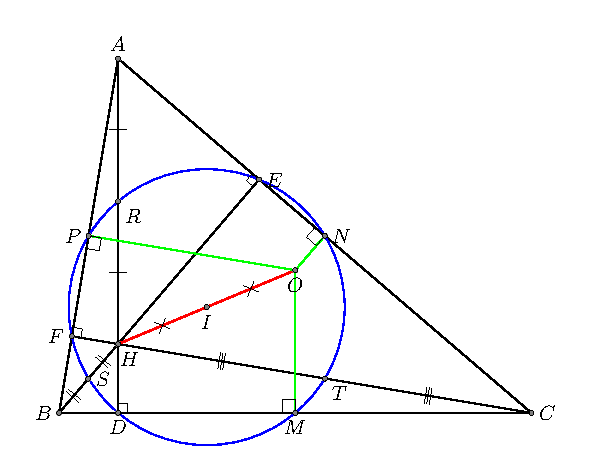
\includegraphics[height=4.5cm]{triangle_euler.pdf}} % instead of \logo 
\institute {\\
\par Tiep Vu Huu\\ \vspace{4mm}}

\begin{document}
%----------- titlepage ----------------------------------------------%
% \begin{frame}[plain]
%   \titlepage 
% \end{frame}

{
\usebackgroundtemplate{\includegraphics[width=\paperwidth]{background_CV.pdf}}%
\begin{frame}[plain]
\end{frame}
}
% section online_editors (end)
\begin{frame}
\frametitle{Online \mylatex editors}
\begin{itemize}
  \item \href{https://www.sharelatex.com/}{\color{blue} ShareLatex }
  \item \href{https://www.overleaf.com/}{\color{blue} Overleaf}
\end{itemize}
No installation required. \\
Provides several templetes.\\
Integrate your account to Dropbox, Github. 
\end{frame}
% =========================== New Slide =================================
\begin{frame}
\frametitle{Start your own CV}
\begin{itemize}
    \item \href{https://www.sharelatex.com/}{\color{blue} ShareLatex }
  \item \href{https://www.overleaf.com/}{\color{blue} Overleaf}

  \item \href{https://github.com/tiepvupsu/LatexBasics}{\tcb My CV's templete} (link is also in the video description below.)
\end{itemize}

\end{frame}
% =========================== New Slide =================================
\begin{frame}[fragile]
\frametitle{Some basic commands/macros}
\begin{itemize}
\item \textit{italic} or {\it italic}
  \begin{lstlisting}
  \textit{italic} or {\it italic}
  % or Ctrl + I in TeX Maker
 \end{lstlisting}

\item \textbf{bold} or {\bf bold}
  \begin{lstlisting}
  \textbf{bold} or {\bf bold}
  % or Ctrl + B in TeX Maker 
 \end{lstlisting}
 \item \textbf{\textit{bold italic}}
 \begin{lstlisting}
  \textbf{\textit{bold italic}} 
  % {\bf {\it bold italic}} behaves differently (try this)
 \end{lstlisting}
\end{itemize}
\end{frame}

% =========================== New Slide =================================
\begin{frame}[fragile]
\frametitle{Some basic commands/macros (con't)}
\begin{itemize}
 % --------------------------------------------------------------
 \item \underline{underline}
 \begin{lstlisting}
  \underline{underline}
  % Ctrl + U in TeX Maker doesn't work!
 \end{lstlisting}
 % --------------------------------------------------------------
 \item \href{https://www.sharelatex.com/learn/Hyperlinks}{\tcb Insert a hyperlink}
 \begin{lstlisting}
  \href{https://www.sharelatex.com/learn/Hyperlinks}
  {\color{blue} Insert a hyperlink}
  % \usepackage{hyperref}
 \end{lstlisting}

 % --------------------------------------------------------------
 \item clickable email to \href{mailto:abc@xyz.com}{a name}.
\begin{lstlisting}
 clickable email to \href{mailto:abc@xyz.com}{a name}.
 \end{lstlisting}

\end{itemize}
\end{frame}

% =========================== New Slide =================================
\begin{frame}[fragile]
\frametitle{Some basic commands/macros (con't)}
\begin{itemize}
 % --------------------------------------------------------------
 \item left alignment \hfill right alignment
 \vspace{-.1in}
  \begin{lstlisting}
  left alignment \hfill right alignment
  % e.g. golden medal in IMO                         2000
 \end{lstlisting}
 % --------------------------------------------------------------
 \item black bullet list 
 \vspace{-.1in}
 \begin{lstlisting}
  \begin{outerlist}
    \item ...
    \item ...
  \end{outerlist}
 \end{lstlisting}
 % --------------------------------------------------------------
 \item white bullet list 
 \vspace{-.1in}
 \begin{lstlisting}
  \begin{innerlist}
    \item ...
    \item ...
  \end{innerlist}
 \end{lstlisting}
\end{itemize}
\end{frame}
% % =========================== New Slide =================================
% \begin{frame}
% \frametitle{Start your own CV}
% \begin{itemize}
%     \item \href{https://www.sharelatex.com/}{\color{blue} ShareLatex }
%   \item \href{https://www.overleaf.com/}{\color{blue} Overleaf}

%   \item \href{https://github.com/tiepvupsu/LatexBasics}{\tcb My CV's templete} (link is also in the video description below.)
% \end{itemize}

% \end{frame}
% =========================== New Slide =================================
% section sources (end)
%\section{Sources} % (fold)
\label{aaa}
\begin{frame}
\frametitle{\mylatex Sources for learning \mylatex}
\begin{itemize}
  \item \href{https://en.wikibooks.org/wiki/LaTeX}{\color{blue} Wikibooks \mylatex}.
  \medskip
  \item \href{https://www.sharelatex.com/learn}{\tcb ShareLaTeX learn}.
  \medskip 

  \item \href{http://tex.stackexchange.com/}{TeX Stack Exchange}.

  \item Google.
  \item \dots 
\end{itemize}
\end{frame}
% % subsection defining_points (end)

% % section points (end)
% % =========================== New Slide =================================
% \begin{frame}[fragile]
% \frametitle{tkz-euclide}

% \begin{columns}
% \begin{column}{0.5\textwidth}
% \begin{itemize}

% \item documentclass
% \vspace{-.2in}

%   \begin{lstlisting}
% \documentclass{standalone} 
% %\documentclass{article}
% \end{lstlisting}

% \item package
% \vspace{-.2in}
% \begin{lstlisting}
% \usepackage{tkz-euclide}
% \usetkzobj{all}
% \end{lstlisting}

% \item main body
% \vspace{-.2in}
% \begin{lstlisting}
% \begin{document}
% % \begin{figure}
% \begin{tikzpicture}
%    ....
% \end{tikzpicture}
% % \end{figure}
% \end{document}
%   \end{lstlisting}
% \end{itemize}
% \href{http://www.altermundus.fr/downloads/documents/Sangaku.pdf}{\color{blue} See tkz-euclide examples here.}
% \end{column}
% \begin{column}{0.5\textwidth}  %%<--- here
%   \centering
%   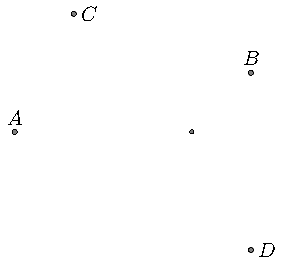
\includegraphics{point1.pdf}
% \end{column}
% \end{columns}
% \end{frame}
% % =========================== New Slide =================================
% % \begin{frame}[fragile]
% % \frametitle{Points}

% % \begin{columns}
% % \begin{column}{0.6\textwidth}
% %   \begin{lstlisting}
% % %% point1.tex
% % ...
% % \begin{document}
% % \begin{tikzpicture}
% %    % defining 1 point
% %    \tkzDefPoint(-3,0){A}
% %    % defining multiple points 
% %    \tkzDefPoints{1/1/B, -2/2/C, 1/-2/D}
% %    % drawing points as dots
% %    \tkzDrawPoints(A,B)
% %    % labeling points
% %    \tkzLabelPoints[above](A,B)
% %    \tkzLabelPoints[right](C,D)
% % \end{tikzpicture}
% % \end{document}
% %   \end{lstlisting}
% % \end{column}
% % \begin{column}{0.4\textwidth}  %%<--- here
% %   \centering
% %   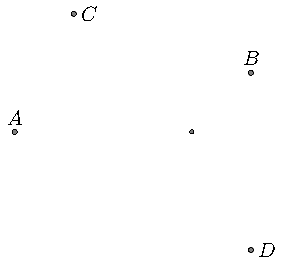
\includegraphics{point1.pdf}
% % \end{column}
% % \end{columns}
% % \end{frame}

% % =========================== New Slide =================================
% %\section{Points} % (fold)
% \label{sec:points}

% \begin{frame}
%   \frametitle{}
% \begin{center}
% \Large{{\color{black}  Learn \mylatex \\Drawing geometric objects with tkz-euclide package}}\\
% \Huge{{\color{blue}  Points}}\\
% \vspace{.1in}
% 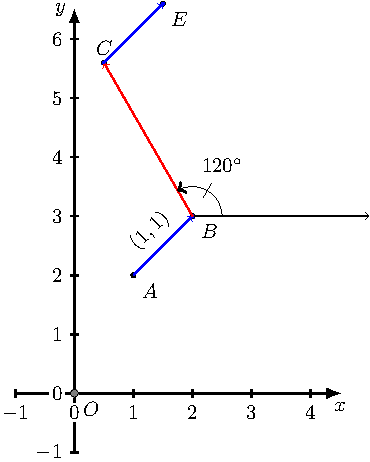
\includegraphics[scale = .7]{relative_coordinate.pdf}
% \par \large{{\color{black}  Tiep Vu Huu}}
% \end{center}
% \end{frame}

% % =========================== New Slide =================================
% \subsection{Points in Cartesian coordinate system} % (fold)
% \label{sub:defining_points}

% \begin{frame}[fragile]
% \frametitle{Points in Cartesian coordinate system}

% \begin{columns}
% \begin{column}{0.5\textwidth}
%   \begin{lstlisting}
% %% def_point_Cartesian.tex
% ...
% \begin{document}
% \begin{tikzpicture}
%    ...
%    % Cartesian coordinate (x,y)
%    \coordinate (O) at (0, 0);
%    \coordinate (A) at (1, 2);
%    % using tkz-euclide
%    \tkzDefPoint(1,1){C}
%    \tkzDefPoints{-1/2/D, 2/-3/E}
%    ...
% \end{tikzpicture}
% \end{document}
%   \end{lstlisting}
%   \href{http://www.highschoolmathandchess.com/latex/altermundus-packages/points-lines-line-segments-rays-and-labels/}{\color{blue} See more here.}
% \end{column}
% \begin{column}{0.5\textwidth}  %%<--- here
%   \centering
%   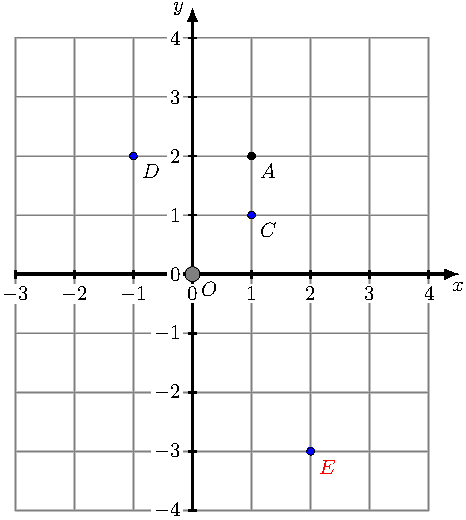
\includegraphics[scale = .7]{def_point_Cartesian.pdf}
% \end{column}

% \end{columns}
% \end{frame}


% % =========================== New Slide =================================
% % subsection polar_coordinate_system (end)
% \begin{frame}[fragile]
% \frametitle{Drawing and Labeling points}

% \begin{columns}
% \begin{column}{0.65\textwidth}
%   \small{\begin{lstlisting}
% %% draw_label_points.tex
% ...
% \begin{tikzpicture}
%   ...
%   % drawing points
%   \tkzDrawPoints(O)
%   \tkzDrawPoints[size=3, fill=black](A)
%   \tkzDrawPoints[size=3, fill=blue](D,E)
%   % labeling points
%   \tkzLabelPoints(O,A,D)
%   \tkzLabelPoints[red](E)
%   % labeling in mathmode
%   \tkzDefPoint[label = below:$A_2$](1,1){A2}
%   \tkzDrawPoints[size=3, fill=blue](A2)
% \end{tikzpicture}
%     \end{lstlisting}}
% \end{column}
% \begin{column}{0.4\textwidth}  %%<--- here
%   \centering
%   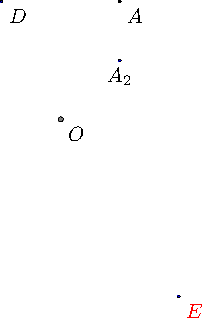
\includegraphics[scale = 1]{draw_label_points.pdf}
% \end{column}
% \end{columns}
% \end{frame}
% % =========================== New Slide =================================
% \subsection{Polar coordinate system} % (fold)
% \label{sub:polar_coordinate_system}

% % subsection polar_coordinate_system (end)
% \begin{frame}[fragile]
% \frametitle{Points in polar coordinate system}

% \begin{columns}
% \begin{column}{0.5\textwidth}
%   \begin{lstlisting}
% %% def_point_polar.tex
% ...
% \begin{document}
% \begin{tikzpicture}
%    ...
%    \coordinate (O) at (0, 0);
%    % polar coordinate, (theta:r)
%    \coordinate (A) at (30:2);
%    \coordinate (B) at (-60:1);

%    \tkzDefPoint(120:1.5){C}
%    ...
% \end{tikzpicture}
% \end{document}
%   \end{lstlisting}
% \end{column}
% \begin{column}{0.5\textwidth}  %%<--- here
%   \centering
%   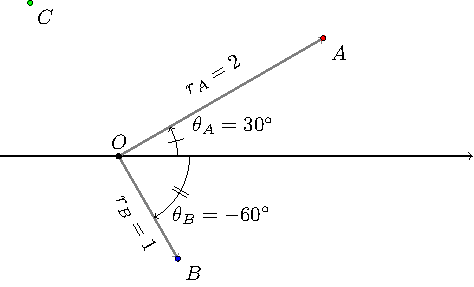
\includegraphics[scale = .7]{def_point_polar.pdf}
% \end{column}
% \end{columns}
% \end{frame}

% % =========================== New Slide =================================
% \subsection{Relative coordinates} % (fold)
% \label{sub:polar_coordinate_system}

% % subsection polar_coordinate_system (end)
% \begin{frame}[fragile]
% \frametitle{Relative coordinates}

% \begin{columns}
% \begin{column}{0.6\textwidth}
%   \begin{lstlisting}
% %% relative_coordinate.tex
% % ...
% \usepackage{calc}
% \begin{document}
% \begin{tikzpicture}
%    % ...
%    \coordinate (O) at (0, 0);
%    \coordinate (A) at (1, 2);
%    \coordinate (B) at ($(A) + (1, 1)$);
%    \coordinate (C) at ($(B) + (120:3)$);
%    \coordinate (E) at ($(C)+(B)-(A)$);
%    % ...
% \end{tikzpicture}
% \end{document}
%   \end{lstlisting}
% \end{column}
% \begin{column}{0.4\textwidth}  %%<--- here
%   \centering
%   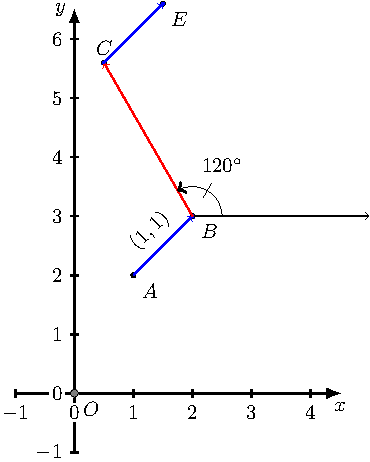
\includegraphics[scale = .7]{relative_coordinate.pdf}
% \end{column}
% \end{columns}
% \end{frame}

% % % =========================== New Slide =================================
% % \begin{frame}[fragile]
% % \frametitle{Points with customized macros}

% % \begin{columns}
% % \begin{column}{0.6\textwidth}
% % \begin{itemize}
% % \item newcommands
% % \end{itemize}
% % \vspace{-.2in}
% % \begin{lstlisting}
% % \newcommand{\myShowPoints}[2]{
% % \tkzDrawPoints(#1) 
% % \tkzLabelPoints[#2](#1)        
% % \end{lstlisting}

% % \begin{itemize}
% % \item main
% % \vspace{-.2in}
% % \hspace{-.5in}
% % \end{itemize}  
% %   \begin{lstlisting}
% % %% point1_2.tex
% % ...
% % %%  newcommands 
% % }       
% % \begin{document}
% % \begin{tikzpicture}
% %    \tkzDefPoint(-3,0){A}
% %    \tkzDefPoints{1/1/B, -2/2/C, 1/-2/D}
% %    % \tkzDrawPoints(A,B,C,D)
% %    % \tkzLabelPoints[above](A,B)
% %    % \tkzLabelPoints[right](C,D)
% %    \myShowPoints{A,B}{left}
% %    \myShowPoints{C,D}{below}
% % \end{tikzpicture}
% % \end{document}
% %   \end{lstlisting}
% % \end{column}
% % \begin{column}{0.4\textwidth}  %%<--- here
% %   \begin{figure}[h]
% %   \centering
% %     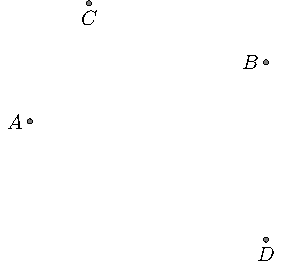
\includegraphics{point1_2.pdf}
% %   \end{figure}
% % \end{column}
% % \end{columns}
% % \end{frame}
% %% ==============================================================
% %\section{Lines, Segments, Rays} % (fold)
% \label{sec:Lines, Segments, Rays}

% \begin{frame}
%   \frametitle{}
% \begin{center}
% \Large{{\color{black}  Learn \LaTeX \\Drawing geometric objects with tkz-euclide package}}\\
% \Huge{{\color{blue}  Lines, Segments, Rays}}\\
% % \vspace{1in}
% 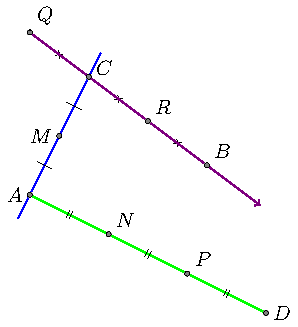
\includegraphics{ratio_point.pdf}
% \par \large{{\color{black}  Tiep Vu Huu}}
% \end{center}
% \end{frame}

% % =========================== New Slide =================================
% \subsection{Connect points} % (fold)
% \label{sub:connect_points}

% % subsection connect_points (end)
% \begin{frame}[fragile]
% \frametitle{Line, Segment, Ray, connecting two points}
% \begin{columns}
% \begin{column}{0.6\textwidth}
%   \begin{lstlisting}
% %% line_segment_ray.tex
% \begin{tikzpicture}
%    % ...
%    % drawing red segments
%    \tkzDrawSegments[red, thick](A,B C,D)
%    % drawing dashed green segment
%    \tkzDrawSegments[green,dashed](A,D)
%    % drawing blue line
%    \tkzDrawLines[draw=blue](A,C B,D)
%    % array with arrow
%    \tkzDrawLines[add = 0 and 0.3, draw=violet, arrows=->](C,B)
%    % ...
% \end{tikzpicture}
% \end{lstlisting}
% \href{http://www.highschoolmathandchess.com/latex/altermundus-packages/points-lines-line-segments-rays-and-labels/}{\color{blue} See more here.}
% \end{column}
% \begin{column}{0.4\textwidth}  %%<--- here
%   \begin{figure}[h]
%   \centering
%     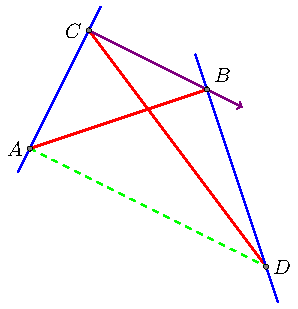
\includegraphics{line_segment_ray.pdf}
%   \end{figure}
% \end{column}
% \end{columns}
% \end{frame}

% % =========================== New Slide =================================
% % \subsection{Labeling and Markers } % (fold)
% % \label{sub:labeling_and_markers_}

% % subsection labeling_and_markers_ (end)
% \begin{frame}[fragile]
% \frametitle{Labeling and Markers}
% \begin{columns}
% \begin{column}{0.6\textwidth}
%   \begin{lstlisting}
% %% lsr_label_marker.tex
% \begin{tikzpicture}
%    % ...
%    % labeling
%    \tkzLabelSegment[above=1pt, rotate=65](A,C){3 cm}
%    \tkzLabelSegment[above=0pt, rotate=-25](A,D){6 cm}
%    % markers
%    \tkzMarkSegment[mark=|](A,C)
%    \tkzMarkSegment[mark=||](A,B)
%    \tkzMarkSegment[mark=|||, size = 2](C,D)
%    \tkzMarkSegment[mark=x](B,D) 
%    % ...
% \end{tikzpicture}
% \end{lstlisting}
% \end{column}
% \begin{column}{0.4\textwidth}  %%<--- here
%   \begin{figure}[h]
%   \centering
%     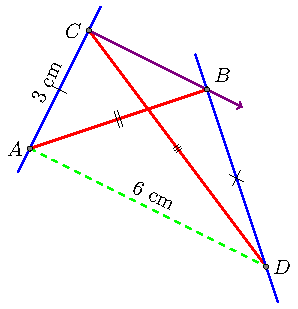
\includegraphics{lsr_label_marker.pdf}
%   \end{figure}
% \end{column}
% \end{columns}
% \end{frame}
% % =========================== New Slide =================================
% % \subsection{Ratio points} % (fold)
% % \label{sub:ratio_points}

% % subsection ratio_points (end)
% \begin{frame}[fragile]
% \frametitle{Define a point between two points for a given length ratio}
% \begin{columns}
% \begin{column}{0.6\textwidth}
%   \begin{lstlisting}
% %% ratio_point.tex
% \begin{tikzpicture}
%    % ...
%    % middle points 
%    \tkzDefMidPoint(A,C)\tkzGetPoint{M}    
%    % others 
%    \coordinate (N) at ($(A)!1/3!(D)$);
%    \coordinate (P) at ($(A)!2/3!(D)$);
%    \coordinate (Q) at ($(C)!-1/2!(B)$);
%    \coordinate (R) at ($(C)!1/2!(B)$);
%    % ...
% \end{tikzpicture}
% \end{lstlisting}
% \end{column}
% \begin{column}{0.4\textwidth}  %%<--- here
%   \begin{figure}[h]
%   \centering
%     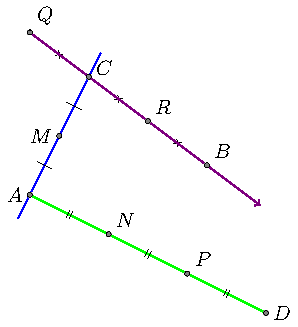
\includegraphics{ratio_point.pdf}
%   \end{figure}
% \end{column}
% \end{columns}
% \end{frame}
% % =========================== New Slide =================================
% % \begin{frame}[fragile]
% % \frametitle{Middle point and markers}
% % \begin{columns}
% % \begin{column}{0.6\textwidth}
% %   \begin{lstlisting}
% % %% midpoint_marker.tex
% % \begin{tikzpicture}
% %    %% defining points and lines 
% %    % middle point 
% %    \tkzDefMidPoint(A,C)\tkzGetPoint{M}
% %    % mark segment
% %    \tkzMarkSegment[mark=|](A,M)
% %    \tkzMarkSegment[mark=|](C,M)
% %    \tkzMarkSegment[mark=||](A,B)
% %    \tkzMarkSegment[mark=x](B,D)
% %    %% showing points
% % \end{tikzpicture}
% % \end{lstlisting}
% % \end{column}
% % \begin{column}{0.4\textwidth}  %%<--- here
% %   \begin{figure}[h]
% %   \centering
% %     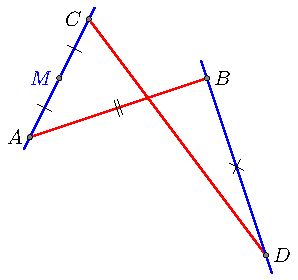
\includegraphics{midpoint_marker.pdf}
% %   \end{figure}
% % \end{column}
% % \end{columns}
% % \end{frame}



% % =========================== New Slide =================================
% \subsection{Intersections} % (fold)
% \label{sub:intersections}
% \begin{frame}[fragile]
% \frametitle{Intersection of two lines}
% \begin{columns}
% \begin{column}{0.6\textwidth}
%   \begin{lstlisting}
% %% intersection1.tex
% ...
% \begin{tikzpicture}
%    %% defining points 
%    % InterLL for intersection of `Line' and `Line'
%    \tkzInterLL(A,B)(C,D) \tkzGetPoint{I}
%    \tkzInterLL(A,C)(B,D) \tkzGetPoint{J}
%    %% showing points
% \end{tikzpicture}
% \end{lstlisting}
% \end{column}
% \begin{column}{0.4\textwidth}  %%<--- here
%   \begin{figure}[h]
%   \centering
%     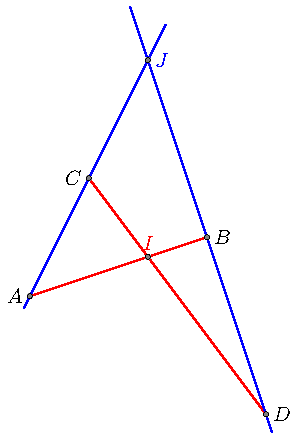
\includegraphics{intersection1.pdf}
%   \end{figure}
% \end{column}
% \end{columns}
% \end{frame}


% % subsection intersections (end)


% \subsection{Orthogonal and Parallel} % (fold)
% \label{sub:Orthogonal and Parallel}
% % =========================== New Slide =================================
% \begin{frame}[fragile]
% \frametitle{Orthogonal and Parallel lines}
% \begin{columns}
% \begin{column}{0.65\textwidth}
%   \begin{lstlisting}
% %% orthogonal_parallel.tex
% ...
% \begin{tikzpicture}
%    % ...
%    %% orthogonal
%    \tkzDefPointBy[projection=onto C--D](A) 
%    \tkzGetPoint{H}
%    \tkzDefLine[orthogonal=through B](C,D) 
%    \tkzGetPoint{K}
%    %% parallel 
%    \tkzDefLine[parallel=through B](C,D)
%    \tkzDrawLine[draw = red, add = .5 and -.6](B,tkzPointResult)
%    % ...
% \end{tikzpicture}
% \end{lstlisting}
% \end{column}
% \begin{column}{0.3\textwidth}  %%<--- here
%   \begin{figure}[h]
%   \centering
%     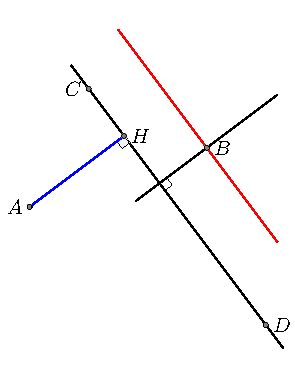
\includegraphics[scale = .8]{orthogonal_parallel.pdf}
%   \end{figure}
% \end{column}
% \end{columns}
% \end{frame}


% %% ==============================================================
% \section{Angles} % (fold)
% \label{sec:Angles}

% \begin{frame}
%   \frametitle{}
% \begin{center}
% \Large{{\color{black}  Learn \LaTeX \\Drawing geometric objects with tkz-euclide package}}\\
% \Huge{{\color{blue}  Angles}}\\
% % \vspace{1in}
% 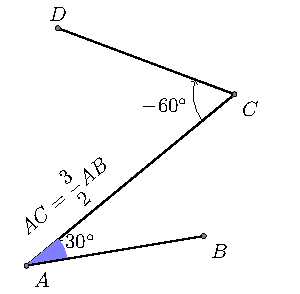
\includegraphics{angle.pdf}
% \par \large{{\color{black}  Tiep Vu Huu}}
% \end{center}
% \end{frame}
% % =========================== New Slide =================================
% \subsection{Specifying angle} % (fold)
% \label{sub:specifying_angle}

% % subsection specifying_angle (end)
% \begin{frame}[fragile]
% \frametitle{Angles}
% \begin{columns}
% \begin{column}{0.6\textwidth}
%   \begin{lstlisting}
% %% angle.tex
% ...
% \begin{tikzpicture}
%    % ...
%   \coordinate (C) at ($(A)!1.5!30:(B)$);
%   \coordinate (D) at ($(C)!.7!-60:(A)$);
%    % ...
% \end{tikzpicture}
% \end{lstlisting}
% \end{column}
% \begin{column}{0.4\textwidth}  %%<--- here
%   \begin{figure}[h]
%   \centering
%     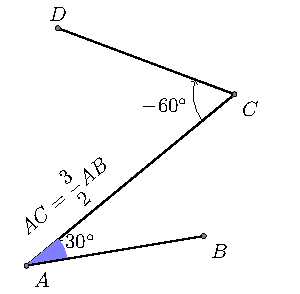
\includegraphics{angle.pdf}
%   \end{figure}
% \end{column}
% \end{columns}
% \end{frame}
% % =========================== New Slide =================================
% \subsection{Labeling and Markers} % (fold)
% \label{sub:specifying_angle}

% % subsection specifying_angle (end)
% \begin{frame}[fragile]
% \frametitle{Labeling and Markers}
% \begin{columns}
% \begin{column}{0.6\textwidth}
%   \begin{lstlisting}
% %% angle_label_marks.tex
% ...
% \begin{tikzpicture}
%    % ...
%    % marker
%    \tkzMarkAngle[size = .5, fill = red!30](B,A,C)
%    \tkzMarkAngle[size = .5, mark = ||,mksize=2](A,C,H)
%    % labeling
%    \tkzLabelAngle[pos=.8](B,A,C){ $60^\circ$}
%    \tkzLabelAngle[pos=1.2,scale = .6](A,C,H){$30^\circ$}
%    % right angle marker
%    \tkzMarkRightAngle[draw =blue](A,H,C)
%    % ...
% \end{tikzpicture}
% \end{lstlisting}
% \end{column}
% \begin{column}{0.4\textwidth}  %%<--- here
%   \begin{figure}[h]
%   \centering
%     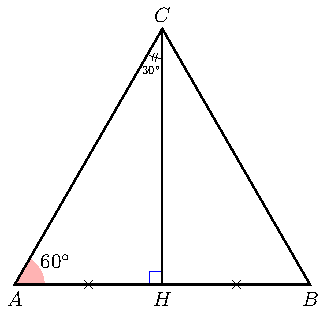
\includegraphics[scale=.9]{angle_label_marks.pdf}
%   \end{figure}
% \end{column}
% \end{columns}
% \end{frame}
% % =========================== New Slide =================================
% \subsection{Angle bisector} % (fold)
% \label{sub:specifying_angle}

% % subsection specifying_angle (end)
% \begin{frame}[fragile]
% \frametitle{Angle Bisector}
% \vspace{-.3in}
% \begin{columns}
% \begin{column}{0.6\textwidth}
%   \begin{lstlisting}
% %% angle_bisector.tex
% ...
% \begin{tikzpicture}
%    % ...
%   \tkzDefLine[bisector](C,B,A) 
%   \tkzGetPoint{i}
  
%   \tkzDrawBisector[draw=blue](C,A,B) 
%   \tkzGetPoint{J}
%    % ...
% \end{tikzpicture}
% \end{lstlisting}
% \end{column}
% \begin{column}{0.4\textwidth}  %%<--- here
%   \begin{figure}[h]
%   \centering
%     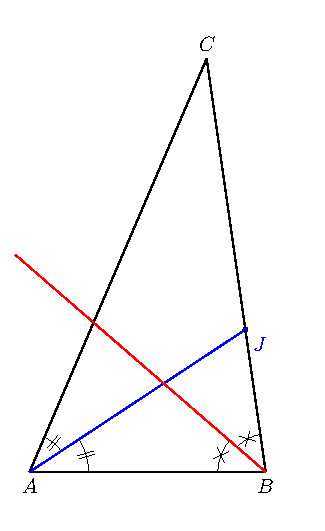
\includegraphics[scale=.9]{angle_bisector.pdf}
%   \end{figure}
% \end{column}
% \end{columns}
% \end{frame}

% %% ==============================================================
% \section{Circles} % (fold)
% \label{sec:Circles}

% % subsection subsection_name (end)
% \begin{frame}
%   \frametitle{}
% \begin{center}
% \Large{{\color{black}  Learn \LaTeX \\Drawing geometric objects with tkz-euclide package}}\\
% \Huge{{\color{blue} Circles}}\\
% \vspace{.1in}
% 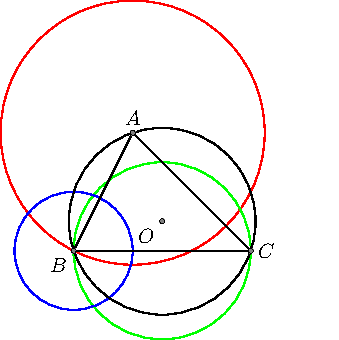
\includegraphics[scale=.9]{circle_1.pdf}
% \par \large{{\color{black}  Tiep Vu Huu}}
% \end{center}
% \end{frame}
% %% ==============New Frame ================================================
% \subsection{Drawing Circles} % (fold)
% \label{sub:specifying_angle}

% % subsection specifying_angle (end)
% \begin{frame}[fragile]
% \frametitle{Drawing Circles}
% \vspace{-.3in}
% \begin{columns}
% \begin{column}{0.6\textwidth}
%   \begin{lstlisting}
% %% circle_1.tex
% ...
% \begin{tikzpicture}
%    % ...
%    % center A, passing B
%    \tkzDrawCircle[draw = red](A,B)
%    % diameter BC
%    \tkzDrawCircle[diameter, draw = green](B,C)
%    % center B, radius 1 cm
%    \tkzDrawCircle[R, draw = blue](B, 1 cm)
%    % passing A, B, C 
%    \tkzDrawCircle[circum](A,B,C)
%    % get its center
%    \tkzCircumCenter(A,B,C)\tkzGetPoint{O}
%    % ...
% \end{tikzpicture}
% \end{lstlisting}
% \href{http://www.highschoolmathandchess.com/latex/altermundus-packages/circles/}{\color{blue}See More Examples here.}
% \end{column}
% \begin{column}{0.4\textwidth}  %%<--- here
%   \begin{figure}[h]
%   \centering
%     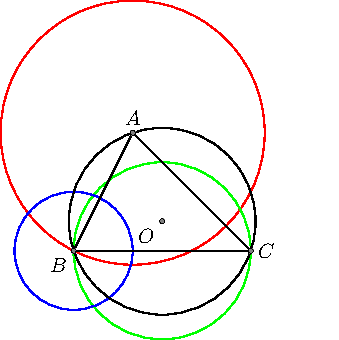
\includegraphics[scale=.9]{circle_1.pdf}
%   \end{figure}
% \end{column}
% \end{columns}
% \end{frame}

% %% ==============New Frame ================================================
% \subsection{Circle Intersection} % (fold)
% \label{sub:specifying_angle}

% % subsection specifying_angle (end)
% \begin{frame}[fragile]
% \frametitle{Circle Intersection}
% \vspace{-.3in}
% \begin{columns}
% \begin{column}{0.6\textwidth}
%   \begin{lstlisting}
% %% circle_intersection.tex
% ...
% \begin{tikzpicture}
%    % ...
%    % Line-Circle intersection
%    \tkzInterLC(C,D)(A,B) 
%    \tkzGetPoints{E}{F}
%    % Circle-Circle intersection
%    \tkzInterCC(A,B)(I,J) 
%    \tkzGetPoints{G}{H}
%    % ...
% \end{tikzpicture}
% \end{lstlisting}
% \href{http://www.highschoolmathandchess.com/latex/altermundus-packages/circles/}{\color{blue}See More Examples here.}
% \end{column}
% \begin{column}{0.4\textwidth}  %%<--- here
%   \begin{figure}[h]
%   \centering
%     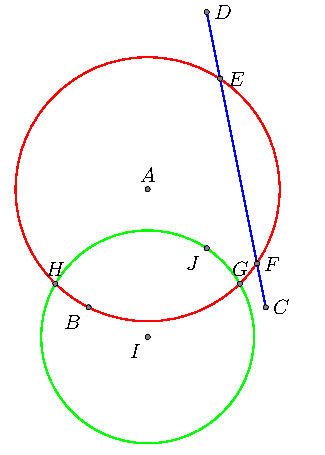
\includegraphics[scale=.9]{circle_intersection.pdf}
%   \end{figure}
% \end{column}
% \end{columns}
% \end{frame}

% %% ==============New Frame ================================================
% \subsection{Circle and Tangents} % (fold)
% \label{sub:specifying_angle}

% % subsection specifying_angle (end)
% \begin{frame}[fragile]
% \frametitle{Circle and Tangents}
% \vspace{-.3in}
% \begin{columns}
% \begin{column}{0.6\textwidth}
%   \begin{lstlisting}
% %% circle_tangent.tex
% ...
% \begin{tikzpicture}
%    % ...
%    \tkzDrawCircle[draw = red](A,B)
%    % from a point on the circle
%    \tkzTangent[at=B](A) \tkzGetPoint{h}
%    % from a point outside the circle
%    \tkzTangent[from=C](A,B) 
%    \tkzGetPoints{M}{N}
%    % ...
% \end{tikzpicture}
% \end{lstlisting}
% \href{http://www.highschoolmathandchess.com/latex/altermundus-packages/circles/}{\color{blue}See More Examples here.}
% \end{column}
% \begin{column}{0.4\textwidth}  %%<--- here
%   \begin{figure}[h]
%   \centering
%     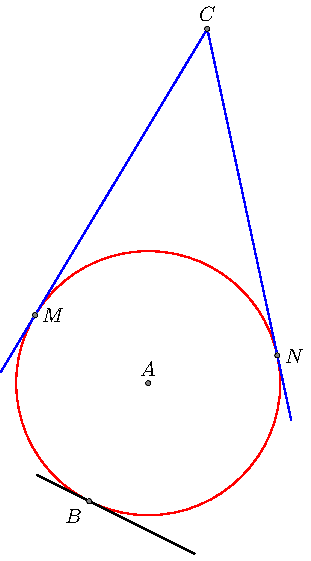
\includegraphics[scale=.8]{circle_tangent.pdf}
%   \end{figure}
% \end{column}
% \end{columns}
% \end{frame}
% % section circle (end)

% %% ==============================================================
% \section{Triangles} % (fold)
% \label{sec:Triangles}

% % subsection subsection_name (end)
% \begin{frame}
%   \frametitle{}
% \begin{center}
% \Large{{\color{black}  Learn \LaTeX \\Drawing geometric objects with tkz-euclide package}}\\
% \Huge{{\color{blue} Triangles}}\\
% \vspace{.1in}
% 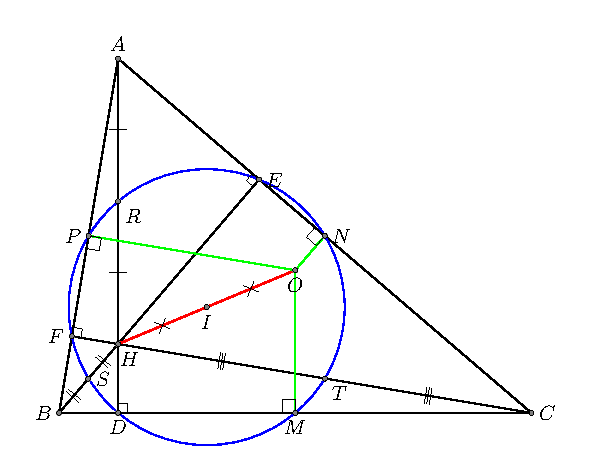
\includegraphics[scale=.6]{triangle_euler.pdf}
% \par \large{{\color{black}  Tiep Vu Huu}}
% \end{center}
% \end{frame}

% \subsection{Drawing triangles} % (fold)
% \label{sub:drawing_triangles}
% %% ==============New Frame ================================================
% % subsection specifying_angle (end)
% \begin{frame}[fragile]
% \frametitle{Drawing triangles}
% \vspace{-.3in}
% \begin{columns}
% \begin{column}{0.6\textwidth}
%   \begin{lstlisting}
% %% triangle_1.tex
% ...
% \begin{tikzpicture}
%    % ...
%    % connecting 3 points
%    \tkzDrawPolygon(A,B,C)
%    % equilateral triangles
%    \tkzDefTriangle[equilateral](C,B) 
%    \tkzGetPoint{D}
%    \tkzDrawPolygon[fill=green!30](B,C,D)
%    % ...
% \end{tikzpicture}
% \end{lstlisting}
% \end{column}
% \begin{column}{0.4\textwidth}  %%<--- here
%   \begin{figure}[h]
%   \centering
%     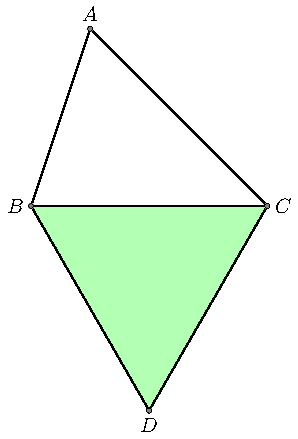
\includegraphics[scale=.8]{triangle_1.pdf}
%   \end{figure}
% \end{column}
% \end{columns}
% \end{frame}

% % subsection specifying_angle (end)
% %% ==============New Frame ================================================
% \subsection{Centroid, Orthocenter, Circumcircle, Inscribed Circle} % (fold)
% \label{sub:centroid_orthocenter_circumcircle_inscribed_circle}

% % subsection centroid_orthocenter_circumcircle_inscribed_circle (end)
% \begin{frame}[fragile]
% \frametitle{Centroid}
% \vspace{-.3in}
% \begin{columns}
% \begin{column}{0.6\textwidth}
%   \begin{lstlisting}
% %% triangle_centroid.tex
% ...
% \begin{tikzpicture}
%    % ...
%    % get centroid
%    \tkzCentroid(A,B,C)\tkzGetPoint{G}
%    % drawing median lines
%    \tkzDrawLines[add = 0 and 1/2](A,G B,G C,G)
%    % ...
% \end{tikzpicture}
% \end{lstlisting}
% \end{column}
% \begin{column}{0.4\textwidth}  %%<--- here
%   \begin{figure}[h]
%   \centering
%     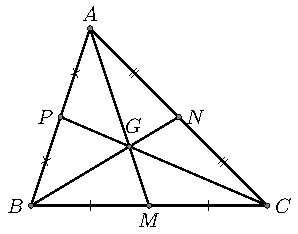
\includegraphics[scale=.8]{triangle_centroid.pdf}
%   \end{figure}
% \end{column}
% \end{columns}
% \end{frame}

% %% ==============New Frame ================================================
% \begin{frame}[fragile]
% \frametitle{Orthocenter}
% % \vspace{-.3in}
% \begin{columns}
% \begin{column}{0.6\textwidth}
%   \begin{lstlisting}
% %% triangle_orthocenter.tex
% ...
% \begin{tikzpicture}
%    % ...
%    % drawing altitudes 
%   \tkzDrawAltitude[draw =blue](B,C)(A) \tkzGetPoint{D}
%   \tkzDrawAltitude[draw =blue](A,C)(B) \tkzGetPoint{E}
%   \tkzDrawAltitude[draw =blue](B,A)(C) \tkzGetPoint{F}
%   % get the orthocenter 
%   \tkzInterLL(A,D)(B,E) \tkzGetPoint{H}
%    % ...
% \end{tikzpicture}
% \end{lstlisting}
% \end{column}
% \begin{column}{0.4\textwidth}  %%<--- here
%   \begin{figure}[h]
%   \centering
%     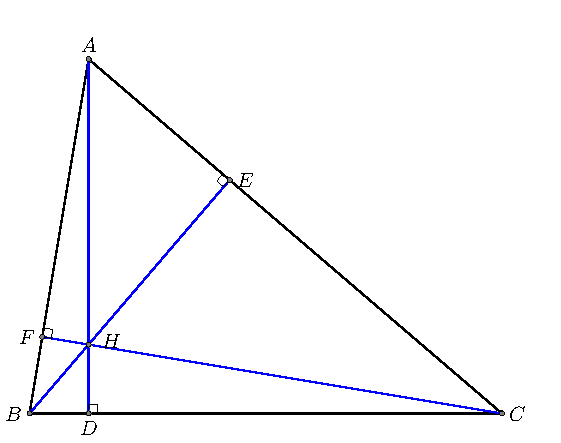
\includegraphics[scale=.5]{triangle_orthocenter.pdf}
%   \end{figure}
% \end{column}
% \end{columns}
% \end{frame}

% %% ==============New Frame ================================================
% \begin{frame}[fragile]
% \frametitle{Circumcircle}
% % \vspace{-.3in}
% \begin{columns}
% \begin{column}{0.6\textwidth}
%   \begin{lstlisting}
% %% triangle_circumcircle.tex
% ...
% \begin{tikzpicture}
%    % ...
%   % draw the circumcircle
%   \tkzDrawCircle[circum](A,B,C)
%   % get its center 
%   \tkzCircumCenter(A,B,C)\tkzGetPoint{O}
%   % draw perpendicular bisector lines 
%   \tkzDrawAltitude[draw =blue](B,C)(O) \tkzGetPoint{D}
%   \tkzDrawAltitude[draw =blue](A,C)(O) \tkzGetPoint{E}
%   \tkzDrawAltitude[draw =blue](B,A)(O) \tkzGetPoint{F}
%    % ...
% \end{tikzpicture}
% \end{lstlisting}
% \end{column}
% \begin{column}{0.4\textwidth}  %%<--- here
%   \begin{figure}[h]
%   \centering
%     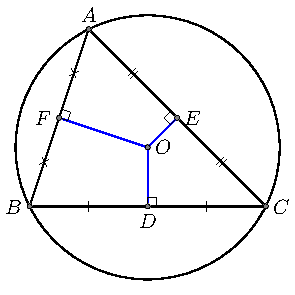
\includegraphics[scale=1]{triangle_circumcircle.pdf}
%   \end{figure}
% \end{column}
% \end{columns}
% \end{frame}

% %% ==============New Frame ================================================
% \begin{frame}[fragile]
% \frametitle{Inscribed circle}
% % \vspace{-.3in}
% \begin{columns}
% \begin{column}{0.6\textwidth}
%   \begin{lstlisting}
% %% triangle_inscribedcircle.tex
% ...
% \begin{tikzpicture}
%    % ...
%   % get the inscbided center 
%   \tkzInCenter(A,B,C) \tkzGetPoint{I}
%   % project it into one edge
%   \tkzDrawAltitude(B,C)(I) \tkzGetPoint{H}
%   % draw the circle 
%   \tkzDrawCircle[draw = red](I,H)
%    % ...
% \end{tikzpicture}
% \end{lstlisting}
% \end{column}
% \begin{column}{0.4\textwidth}  %%<--- here
%   \begin{figure}[h]
%   \centering
%     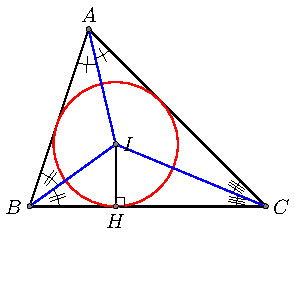
\includegraphics[scale=1]{triangle_inscribedcircle.pdf}
%   \end{figure}
% \end{column}
% \end{columns}
% \end{frame}

% %% ==============New Frame ================================================
% \begin{frame}[fragile]
% \frametitle{Euler circle}
% % \vspace{-.3in}
% \begin{figure}
% \centering
% 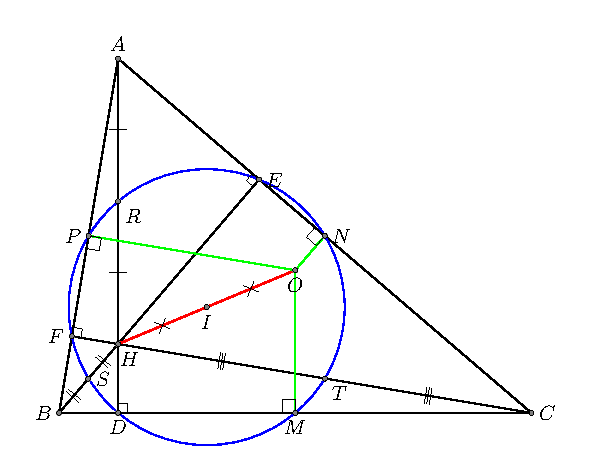
\includegraphics{triangle_euler.pdf}
% \end{figure}
% \end{frame}
% % subsection drawing_triangles (end)
  \begin{frame}
  \vfill
  \centering
  \begin{beamercolorbox}[sep=8pt,center,shadow=true,rounded=true]{title}
    \usebeamerfont{title} Thanks for watching%
  \end{beamercolorbox}
  \vfill
  \end{frame}
\end{document}
